%!BIB program=biber

\documentclass{article} %类型为文章
\usepackage[UTF8]{ctex} %中文编码宏
\usepackage[hidelinks]{hyperref} %超链接宏
\usepackage{geometry} %页面控制宏
\usepackage{fancyhdr} %页眉页脚宏
\usepackage{lastpage} %总计页的宏
\usepackage{color} %颜色控制宏
\usepackage{graphicx} %图片插入宏
\usepackage{subfigure} %子图插入宏
\usepackage{diagbox} %表格斜线宏
\usepackage{multirow} %纵向合并宏
\usepackage{makecell} %表格换行宏
\usepackage{amsmath} %公式插入宏
\usepackage{cases}
\usepackage{unicode-math} %公式样式宏
\usepackage{algorithm2e} %伪代码宏
\usepackage{gbt7714} %国标引用宏
\usepackage{url} %网页链接宏
\usepackage{doi} %doi号宏
\renewcommand{\vec}[1]{\boldsymbol{#1}} %设置向量样式

\usepackage{listings}
\usepackage{color}
\definecolor{dkgreen}{rgb}{0,0.6,0}
\definecolor{gray}{rgb}{0.5,0.5,0.5}
\definecolor{mauve}{rgb}{0.58,0,0.82}
\lstset{frame=tb,
  language=Python,
  aboveskip=3mm,
  belowskip=3mm,
  showstringspaces=false,
  columns=flexible,
  basicstyle={\small\ttfamily},
  numbers=left,%设置行号位置none不显示行号
  %numberstyle=\tiny\courier, %设置行号大小
  numberstyle=\tiny\color{gray},
  keywordstyle=\color{blue},
  commentstyle=\color{dkgreen},
  stringstyle=\color{mauve},
  breaklines=true,
  breakatwhitespace=true,
  escapeinside=``,%逃逸字符(1左面的键),用于显示中文例如在代码中`中文...`
  tabsize=4,
  extendedchars=false %解决代码跨页时,章节标题,页眉等汉字不显示的问题
}

\geometry{a4paper,left=2cm,right=2cm,top=2cm,bottom=2cm,headsep=0.5cm,footskip=1cm} %设置页边距和页眉页脚距离
\pagestyle{fancy} %设置页面样式
\fancyhf{} %开启页眉页脚
\lhead{欧纪阳 2019141220016} %设置左侧页眉为作者
\rhead{Sichuan University 四川大学} %设置右侧页眉为机构
\cfoot{第\thepage 页 \quad 共 \pageref{LastPage} 页} %设置居中页脚为页码

\linespread{1.2} %行距
\setlength{\parskip}{0.5em} %段落间距
\setlength{\parindent}{2em} %缩进距离

\setmathfont{Cambria Math} %设置数学公式样式
\bibliographystyle{gbt7714-numerical} %设置参考文献样式

\title{多重网格-五点差分-共轭梯度法\\——求解二维泊松方程的一类边值问题:\\从电荷分布求解电场的数值方法} %设置标题
\author{欧纪阳 2019141220016\\ \textit{College of Physics, Sichuan University, Chengdu 610064, China}} %设置作者
\date{\today} %设置日期

\begin{document}
\maketitle %插入标题
\begin{abstract} %插入摘要和关键字
    \quad 本文报告了一种在二维空间中求解泊松方程的一类边值问题的方法——多重网格-五点差分-共轭梯度法,该算法为有限差分法的改进方法,利用五点差分法作为数值微分近似,构建对角线稀疏矩阵,以共轭梯度方法为线性系统求解器,采用V循环多重网格方法加速迭代。本文还展示了用Python求解在有限矩形区域内给定电荷分布,并已知电势的边值的条件下的,该区域内的电势和电场分布。相较于高斯-赛德尔、过松弛迭代等求解算法,其收敛速度更快,精度更高。在复杂的边值条件下,与普通网格下的共轭梯度迭代相比,可快速降低误差。

    \textbf{关键词:}多重网格法 \quad 共轭梯度法 \quad 稀疏矩阵 \quad 泊松方程 \quad 边值问题 \quad Python
\end{abstract}

\tableofcontents %插入目录
\thispagestyle{empty} %本页无页眉页码

\newpage

\section{介绍}
求解偏微分方程的数值方法有许多,其步骤大致分为以下几个部分:用差分代替微分,带入边界条件组装系数矩阵,使用合适的线性方程求解器进行求解。以二维泊松方程为例,其只含有两项对相同坐标的二阶偏微分,最常用的差分方法就是对每一个坐标取三点中心差分,对于线性求解迭代方法,主要有雅克比方法、高斯-赛德尔方法、连续过松弛迭代方法、共轭梯度方法等。雅克比方法是线性方程组系统中的一种不动点迭代方法,把系数矩阵$A$分解为主对角线矩阵$D$,上三角矩阵$U$和下三角矩阵$L$,其不动点迭代形式为,
\begin{align}
    x_{i+1}=D^{-1}[b-(L+U)x_i]
\end{align}
其中$b$表示常数项。与雅克比方法紧密相关的迭代方法是高斯-赛德尔方法高斯方法,两者之间的差别是后者最近更新的未知变量的值在每一部中都使用,即使更新发生在当前步骤,其迭代形式为,
\begin{align}
    x_{i+1}=D^{-1}(b-Ux_{i}-Lx_{i+1})
\end{align}
因此其收敛速度常常比雅克比方法更快。连续过松弛方法是使用高斯-赛德尔的求解方向,并使用过松弛加以加快收敛速度,其迭代形式为
\begin{align}
    x_{i+1}=(\omega L+D)^{-1}[(1-\omega)Dx_i-\omega Ux_i]+\omega (D+\omega L)^{-1}b
\end{align}
其中$\omega$成为松弛因子,当$\omega >1$时成为过松弛,对于不同的新系统有不同的$\omega$最优选择。过松弛迭代对于一般的线性系统已经能达到很高的迭代速度,但是对于具有大量零的稀疏矩阵来说,其效率往往较低,例如二维泊松方程,其系数矩阵只在五条对角线上具有非零元素,随着网格的精细,除了迭代速度减慢以外,存储矩阵所需的内存也不断增大,这对计算机的要求大大提高。以上的这些方法都是在确定的网格下进行迭代,也就是说在整个迭代过程中网格的精度是不会变化的,但是在一些系统中,高频信息与低频信息的收敛速度是不一样的,一种解决的思路就是运用层次离散化的方法进行求解。

本文报告了一种求解泊松方程的高效方法:多重网格-五点差分-共轭梯度法。该方法在每一级网格中,首先利用五点差分法对偏微分做近似,将二维偏微分方程改写为一维的线性方程组,根据边界条件组装好系数矩阵后,利用对角稀疏矩阵进行储存,该矩阵为一个对角正定矩阵(或对角负定矩阵),因此可以利用共轭梯度法作为线性求解器进行求解。在迭代求解的过程中运用V循环多重网格方法作为预调节器,现在低精度的网格中进行迭代,再逐步将计算结果插值到更加精细的网格中进行迭代,以达到提高收敛速度,并同时降低高频误差与低频误差的目的。

\section{方法}
报告的方法的最终目的是通过在二维空间中求解泊松方程的边值问题,
\begin{align}
    \nabla^2 \varphi = -\frac{\rho}{\varepsilon} \Rightarrow \frac{\partial^2 \varphi (x,y)}{\partial x^2}+\frac{\partial^2 \varphi (x,y)}{\partial y^2}=f(x,y) \label{3.0}
\end{align}
从而通过$\vec{E}=-\nabla \varphi$求解电场强度矢量。(\ref{3.0})式为一个二阶偏微分方程,计算机无法直接求解,报告的方法实质上是有限差分法的扩展,先通过数值微分将偏微分方程化为线性方程,再在合适的网格上施以合适的线性求解器进行求解。
\subsection{五点差分方法}
在说明二维问题前,先讨论一维数值微分,对于一个三阶可微函数$f(x)$,根据泰勒定理有,
\begin{align}
    f(x+h) & =f(x)+hf'(x)+\frac{h^2}{2}f''(x)+\frac{h^3}{6}f^{(3)}(c_1) \\
    f(x-h) & =f(x)-hf'(x)+\frac{h^2}{2}f''(x)-\frac{h^3}{6}f^{(3)}(c_2)
\end{align}
其中$x-h<c_2<x<c_1<x+h$,最后一项为误差项,两式相减可以得到\textbf{一阶导数的三点中心差分公式},
\begin{align}
    f'(x)=\frac{f(x+h)-f(x-h)}{2h}-\frac{h^2}{6}f^{(3)}(c)=\frac{f(x+h)-f(x-h)}{2h}+O(x^3)
\end{align}
用该公式在离散情况下对$\vec{E}=-\nabla \varphi$做近似可得,
\begin{align}
    \vec{E}_{i,j}=\left(-\frac{\varphi_{i+1,j}-\varphi_{i-1,j}}{2h_x},-\frac{\varphi_{i,j+1}-\varphi_{i,j-1}}{2h_y}\right)
\end{align}
其中$\left\{\varphi_{i,j}|0\leq i\leq m-1,0\leq j\leq n-1\right\}$,$h_x,h_y$分别为$x$方向和$y$方向上的网格精度。

类似地,该方法可以得到更高阶的差分公式,对四阶可微函数$f(x)$,根据泰勒定理有,
\begin{align}
    f(x+h) & =f(x)+hf'(x)+\frac{h^2}{2}f''(x)+\frac{h^3}{6}f^{(3)}(x)+\frac{h^4}{24}f^{(4)}(c_1) \\
    f(x-h) & =f(x)-hf'(x)+\frac{h^2}{2}f''(x)-\frac{h^3}{6}f^{(3)}(x)+\frac{h^4}{24}f^{(4)}(c_2)
\end{align}
其中$x-h<c_2<x<c_1<x+h$,最后一项为误差项,两式相加可以得到\textbf{二阶导数的三点中心差分公式},
\begin{align}
    f''(x)=\frac{f(x-h)-2f(x)+f(x+h)}{h^2}-\frac{h^2}{12}f^{(4)}(c)=\frac{f(x-h)-2f(x)+f(x+h)}{h^2}+O(x^4)
\end{align}

对泊松方程中的两个微分算子在离散情况下,分别应用二阶导数的三点中心差分公式,
\begin{align}
    \frac{\partial^2 \varphi_{i,j}}{\partial x^2} & =\frac{\varphi_{i-1,j}-2\varphi_{i,j}+\varphi_{i+1,j}}{h_x^2} & \frac{\partial^2 \varphi_{i,j}}{\partial y^2} & =\frac{\varphi_{i,j-1}-2\varphi_{i,j}+\varphi_{i,j+1}}{h_y^2}
\end{align}
由于每一个网格的偏微分需要五个网格进行计算,故称为\textbf{五点差分法}。由此便得到了应用五点差分法近似后得到的泊松方程,
\begin{align}
    \frac{\varphi_{i-1,j}+\varphi_{i+1,j}}{h_x^2}-2(\frac{1}{h_x^2}+\frac{1}{h_y^2})\varphi_{i,j}+\frac{\varphi_{i,j-1}+\varphi_{i,j+1}}{h_y^2}=f_{i,j} \label{3.1}
\end{align}

\subsection{系数矩阵的组装}
由于求解的方程是二维的,需要将其重塑回到一维才能求解,
\begin{align}
    u_{i+jm}=a_{i,j},\, \left\{a_{i,j}|0\leq i\leq m-1,0\leq j\leq n-1\right\}
\end{align}
例如对于一个$A_{4\times 4}$的矩阵将会变换为,
\begin{align}
    \begin{bmatrix}
        0  & 1  & 2  & 3  \\
        4  & 5  & 6  & 7  \\
        8  & 9  & 10 & 11 \\
        12 & 13 & 14 & 15
    \end{bmatrix}
    \Rightarrow
    \left[0,1,2,3,4,5,6,7,8,9,10,11,12,13,14,15\right].\mathrm{T}
\end{align}
对于(\ref{3.1})式,$\varphi$与$f$的大小为$(m,n)$,利用以上方法把(\ref{3.1})式改写为$Ax=b$的形式,即$\varphi \rightarrow x, f \rightarrow b ,\nabla^2 \rightarrow A$,其中系数矩阵A为,
\begin{align}
    \footnotesize
    \begin{bmatrix}
        -2(\frac{1}{h_x^2}+\frac{1}{h_y^2}) & \frac{1}{h_x^2}                     & \cdots                              & \frac{1}{h_y^2}                                                                                                                                                                                                                                   \\
        \frac{1}{h_x^2}                     & -2(\frac{1}{h_x^2}+\frac{1}{h_y^2}) & \frac{1}{h_x^2}                     & \cdots                              & \frac{1}{h_x^2}                                                                                                                                                                                             \\
        \vdots                              & \frac{1}{h_x^2}                     & -2(\frac{1}{h_x^2}+\frac{1}{h_y^2}) & \frac{1}{h_x^2}                     & \cdots                                              & \frac{1}{h_y^2}                                                                                                                                       \\
        \frac{1}{h_y^2}                     & \vdots                              & \frac{1}{h_x^2}                     & -2(\frac{1}{h_x^2}+\frac{1}{h_y^2}) & \frac{1}{h_x^2}                                     & \cdots                              & \frac{1}{h_y^2}                                                                                                 \\
                                            & \ddots                              & \ddots                              & \ddots                              & \ddots  \ddots \ddots \ddots  \ddots \ddots  \ddots & \ddots                              & \ddots                              & \ddots                                                                    \\
                                            &                                     & \frac{1}{h_y^2}                     & \cdots                              & \frac{1}{h_x^2}                                     & -2(\frac{1}{h_x^2}+\frac{1}{h_y^2}) & \frac{1}{h_x^2}                     & \vdots                              & \frac{1}{h_y^2}                     \\
                                            &                                     &                                     & \frac{1}{h_y^2}                     & \cdots                                              & \frac{1}{h_x^2}                     & -2(\frac{1}{h_x^2}+\frac{1}{h_y^2}) & \frac{1}{h_x^2}                     & \vdots                              \\
                                            &                                     &                                     &                                     & \frac{1}{h_y^2}                                     & \cdots                              & \frac{1}{h_x^2}                     & -2(\frac{1}{h_x^2}+\frac{1}{h_y^2}) & \frac{1}{h_x^2}                     \\
                                            &                                     &                                     &                                     &                                                     & \frac{1}{h_y^2}                     & \cdots                              & \frac{1}{h_x^2}                     & -2(\frac{1}{h_x^2}+\frac{1}{h_y^2})
    \end{bmatrix} \label{3.2}
\end{align}
那么做变换后得到的$x,b$的大小为为$(1,mn)$,系数$A$矩阵的大小为$(mn,mn)$,矩阵中同一行同一列的$\frac{1}{h_x^2}$与$\frac{1}{h_y^2}$之间的间距为$m-1$,即矩阵中的$\cdots\,\vdots$表示占据$m-2$个元素,并且$1$级、$-1$级副对角线上的元素,从第$m$个元素开始,每隔$m-1$个元素应该为零((\ref{3.2})式中没有体现出来)。例如对于一个$4\times 4$的网格,假设$h_x=h_y=1$,其系数矩阵$A$写作,
\begin{align}
    \addtocounter{MaxMatrixCols}{25}
    \begin{bmatrix}
        -4 & 1  &    &    & 1                                                         \\
        1  & -4 & 1  &    &    & 1                                                    \\
           & 1  & -4 & 1  &    &    & 1                                               \\
           &    & 1  & -4 & 0  &    &    & 1                                          \\
        1  &    &    & 0  & -4 & 1  &    &    & 1                                     \\
           & 1  &    &    & 1  & -4 & 1  &    &    & 1                                \\
           &    & 1  &    &    & 1  & -4 & 1  &    &    & 1                           \\
           &    &    & 1  &    &    & 1  & -4 & 0  &    &    & 1                      \\
           &    &    &    & 1  &    &    & 0  & -4 & 1  &    &    & 1                 \\
           &    &    &    &    & 1  &    &    & 1  & -4 & 1  &    &    & 1            \\
           &    &    &    &    &    & 1  &    &    & 1  & -4 & 1  &    &    & 1       \\
           &    &    &    &    &    &    & 1  &    &    & 1  & -4 & 0  &    &    & 1  \\
           &    &    &    &    &    &    &    & 1  &    &    & 0  & -4 & 1  &    &    \\
           &    &    &    &    &    &    &    &    & 1  &    &    & 1  & -4 & 1  &    \\
           &    &    &    &    &    &    &    &    &    & 1  &    &    & 1  & -4 & 1  \\
           &    &    &    &    &    &    &    &    &    &    & 1  &    &    & 1  & -4 \\
    \end{bmatrix}
\end{align}
显然该矩阵为一个稀疏矩阵,只在主对角线、$1,-1,m,-m$级副对角线五条对角线上有元素,因此在程序中构建此矩阵,并将其储存到内存中时,将应用\textbf{对角稀疏矩阵方法},即内存器只储存非零对角线上的元素,在编写中使用scipy.sparse.dia\_matrix库进行矩阵的存储与运算。

\subsection{添加一类边值条件}
对于(\ref{3.2})式中的矩阵,如果没有加边界条件的话,求解过程会非常缓慢,而且最终的求解结果显示,其等价的边界条件为四个边界均满足$\varphi=0$,因此在求解之前应施加一定的边界条件。在经改写后得到的线性方程组中添加一类边界,($\varphi=\phi(q)$,其中$q$为边界上的坐标),的方法十分简单,只需在系数矩阵$A$中找到边界点对应的行,将对角线上的元素该写为1,再将$b$中对应的元素改写为对应的$\phi(q)$即可。

\subsection{共轭梯度方法}
在众多的线性方程求解器中,目前共轭梯度方法是求解稀疏矩阵最优化的方法,特别是在引入有效的预条件后,许多其他方法难以处理的问题使用该方法可以高效的解决,其收敛速度远高于高斯-赛德尔、过松弛迭代等方法,因此在求解线性近似的偏微分方程时,首选使用共轭梯度方法,可以在有限步骤获得线性系统$Ax=b$的解,其伪代码如算法\ref{A1}。
\begin{algorithm}
    \LinesNumbered
    \KwIn{$A$:系数矩阵\newline
        $b$:常数项\newline
        $x_0$:初始预测值}
    $d_0 = r_0 = b-Ax_0$\\
    \For{$k=0,1,2,\cdots,n-1$}{
        \If{$r_k = 0$}{
            \textbf{break}
        }
        $\alpha_k = \frac{r_k^T r_k}{d_k^T A d_k}$\\
        $x_{k+1} = x_k+\alpha_k d_k$\\
        $r_{k+1} = r_k-\alpha_k A d_k$ '计算余项\\
        $\beta = \frac{r_{k+1}^T r_{k+1}}{r_k^T r_k}$
    }
    \KwOut{$x_k$:线性方程组的解}
    \caption{共轭梯度方法}
    \label{A1}
\end{algorithm}

算法\ref{A1}通过使用预条件方法,可以使迭代收敛速度加快,迭代方法的收敛率通常直接或间接依赖于系数矩阵$A$的条件数,预条件方法的思想便是降低问题中的条件数。在对称连续过松弛中,预条件子定义为,
\begin{align}
    M=(D+\omega L)D^{-1}(D+\omega U)
\end{align}
其中$A=L+D+U$被分解为下三角部分、对角线、以及上三角部分,$0<\omega<2$,当$\omega = 1$时被称为高斯-赛德尔与条件子。虽然预条件可以大大的加快迭代的速度,但是如果预条件子矩阵难以求逆,一般情况下反而会适得其反,故在本文中运用的是无预条件的共轭梯度方法。

\subsection{多重网格方法}
在数值分析中,多重网格法是一种使用层次离散化来求解微分方程的方法,是多分辨率方法的一个例子。由于直接在高分辨率(用于求解的间隔小)上进行求解时对于低频部分收敛较慢,与间隔的平方成反比,便想可以到先在低分辨率(间隔较大)上进行求解,然后再进行插值,提高其分辨率,再在更高分辨率进行计算,这样的方法就叫做多重网格方法,且迭代过程主要包含以下几个重要的组成部分:
\begin{itemize}
    \item 平滑(smoothing):用线性求解器进行迭代,降低高频误差。
    \item 计算残差(Residual Computation):在平滑之后计算剩余误差(残差)$r_i=b-Ax_i$。
    \item 限制(Restriction):降低采样率,把残差放到更加粗糙的网格中。
    \item 延拓(prolongation):将粗网格计算的修正值插值到更精细的网格中
    \item 修正(Correction):将延拓的修正值添加到精细网格中。
\end{itemize}

多重网格方法有多种变体,但均包含以上步骤,在本文中运用的是最基础的\textbf{V循环多重网格方法},因其迭代过程为逐次预光滑降低到最粗糙的网格中,再逐次求解插值到最精细的网格中,所形成的迭代图像为一个“V”字形,故得名V循环多重网格方法,其重要步骤如算法\ref{A2},也可以用图\ref{F0}来表示:
\begin{algorithm}
    \LinesNumbered
    \KwIn{$\varphi$:初始预测值\newline
        $f$:常数项\newline
        $h$:最精细网格精度\newline
        $h_m$:最粗糙网络精度}
    \SetKwFunction{VCycle}{VCycle}
    \SetKwFunction{smoothing}{smoothing}
    \SetKwFunction{residual}{residual}
    \SetKwFunction{restriction}{restriction}
    \SetKwFunction{prolongation}{prolongation}
    \SetKwFunction{zeros}{zeros}
    \SetKwFunction{size}{size}
    \SetKwProg{Fn}{Function}{:}{end}
    \Fn{\VCycle{$\varphi,f,h$}}{
        $\varphi$ = \smoothing{$\varphi,f,h$} '预平滑(pre-smoothing)\\
        $res$ = \residual{$\varphi,f,h$}\\
        $rhs$ = \restriction($res$)\\
        $eps$ = \zeros(\size($rhs$))\\
        \eIf{$h$ < $h_m$}{
            \VCycle{$eps,rhs,2h$}
        }{
            \smoothing{$eps,rhs,2h$}
        }
        $\varphi$ = $\varphi$ + \prolongation($eps$)\\
        $\varphi$ = \smoothing{$\varphi,f,h$} '后平滑(post-smoothing)\\
        \textbf{return} $\varphi$
    }
    \KwOut{$\varphi$:线性方程组的解}
    \caption{多重网格方法}
    \label{A2}
\end{algorithm}

\begin{figure}
    \begin{center}
        \includegraphics[width=17cm]{Multigrid_Visualization.png}
    \end{center}
    \caption{V循环多重网格方法的示意图}
    \label{F0}
\end{figure}

算法\ref{A2}中,需要先对进入迭代的预测解$\varphi$进行一次预平滑,即使用求解器对其进行较少次数的迭代,使其较靠近精确解,本文使用的求解器为共轭梯度方法,在编写中一般要求在预平滑中迭代$3\sim 5$次即可;插值后进行的后平滑一般按照设定的精度进行,每相邻两级网格之间的网格精度一般是翻一倍,对于求解精度每一级网格设置为相同即可;对于限制算子(Restriction)和延拓(Prolongation)均采用\textbf{双线性插值方法},其为一维两点线性插值的的二维推广方法,限于篇幅,此处不再过多赘述。

\subsection{可视化与误差分析}
对于电势的可视化,本文使用matplotlib.pyplot库中,利用不同颜色来标注大小的pcolor函数来绘制电势在空间中的分布,再使用contour函数绘制其等势线;对于电场的可视化,将在运用pcolor函数来绘制电场强度大小在空间中的分布之外,利用quiver函数辅以$19\times 19$个箭头来表示电场强度矢量的方向。误差分析方面,将对一组拥有解析解情况的泊松方程进行数值计算,并与精确解进行对比,计算均方误差RMS。

\section{结果}
该部分展示了一些数值计算的例子,为了证明该方法的有效性,将会给予一组具有解析解的电荷分布及边值条件进行求解,并与理论上的解析解的结果进行对比,除此之外还将展示点电荷、电偶极子、带点细棍等所产生的电场在有限空间中的分布。

\subsection{二维正弦电荷分布}
利用多重网格-五点差分-共轭梯度法和直接共轭梯度方法(只在一级网格中进行迭代)对以下边值问题进行求解,
\begin{subnumcases}{}
    \frac{\partial^2 \varphi}{\partial x^2}+\frac{\partial^2 \varphi}{\partial y^2}=-\frac{\rho}{\varepsilon}=-2\pi^2 \sin(\pi x)\sin(\pi y)\\
    \varphi=0, \, x=\pm 1  \label{2.1a}\\
    \varphi=0, \, y=\pm 1  \label{2.1b}
\end{subnumcases}
显然该系统具有解析解,并可推导得到电场强度矢量的表达式,
\begin{align}
    \varphi & =\sin(\pi x)\sin(\pi y) & E=-\pi\cos(\pi x)\sin(\pi y)\vec{e_x}+\pi\sin(\pi x)\cos(\pi y)\vec{e_y}
\end{align}

在进行数值计算时,设置求解区域为$S=\left\{(x,y)|-1\leq x\leq 1,-1\leq y\leq 1\right\}$的正方形区域,在两个维度上的网格精度均为$10^{-3}$,即求解区域的网格大小为$2000\times 2000$,调节求解参数,多重网格等级为3,预平滑迭代次数为3,后平滑迭代求解精度为$10^{-10}$。最终求解结果如图\ref{F1}(a)所示,实际计算误差$RMS=4.112377\times 10^{-7}$,数值的后平滑迭代过程在三级网格中经历了1次,在二级网格中经历了7次,在一级网格中经历了43次,包括预平滑、限制、插值、后平滑等所有过程在内的10次平均总耗时约为6.89692s,与直接共轭梯度方法的55次迭代,10次平均总耗时10.2639s相比,误差降低的速度要高出许多,误差下降曲线如图\ref{F1}(b)所示,蓝色曲线从最高一级粗网格后迭代开是记录误差,从第九个数据点开始回到一级精细网格,虽然此处误差较大,但是可以以很快的速度降低误差,因为前8次迭代是在粗化的网格下进行,所以所报告的算法总体效率要高于直接共轭梯度法。
\begin{figure}[ht]
    \begin{center}
        \subfigure[数值计算得到的电势与电场分布]{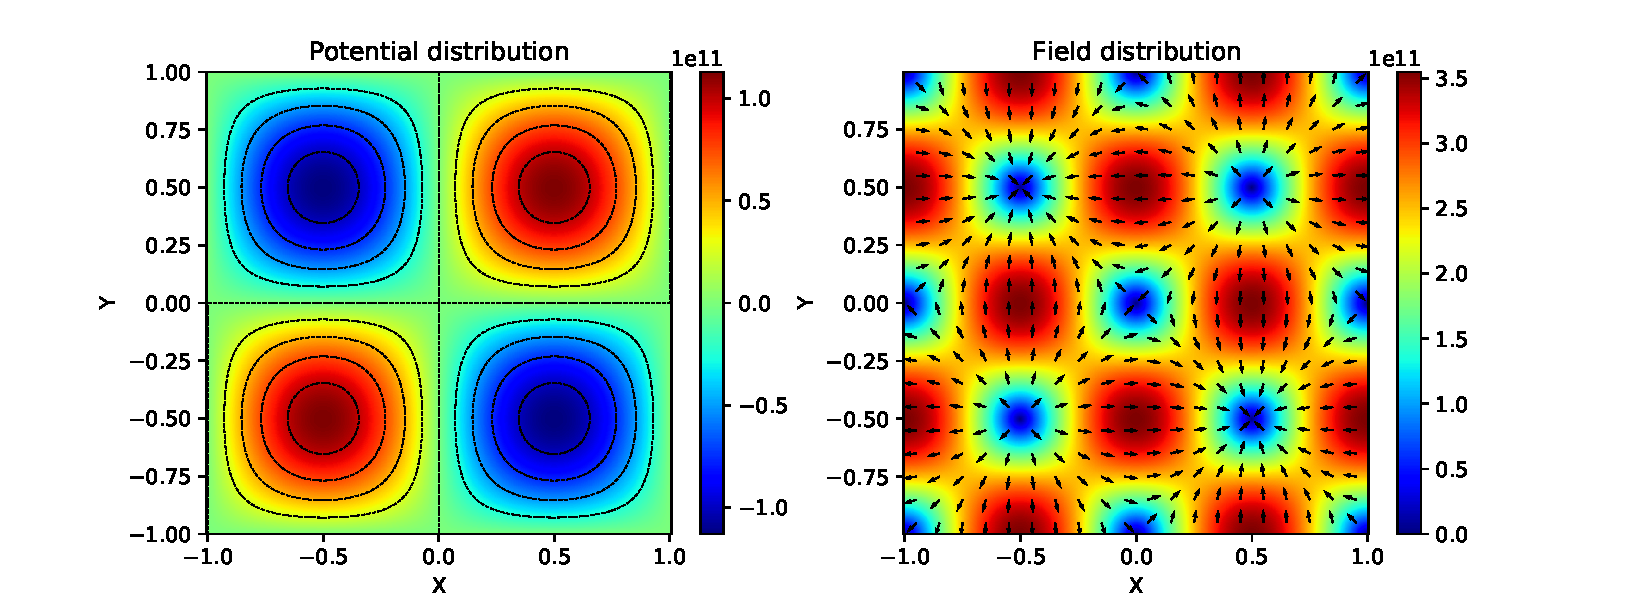
\includegraphics[width=17cm]{q2e.png}}
        \subfigure[误差下降曲线]{\includegraphics[width=17cm]{error.pdf}}
    \end{center}
    \small
    \qquad (a)中左图展示的是电势在求解空间中的分布情况,黑色虚线表示等势面;右图展示的是电场强度在求解空间中的分布情况,颜色的不同表示电场强度大小,箭头表示箭头根部所在的位置的电场强度矢量的方向。(b)为多重网格-共轭梯度法(MG-CGM)后迭代过程(蓝色)、直接共轭梯度法(SG-CGM)(橙色)的误差下降曲线。
    \caption{二维正弦电荷分布的数值计算结果}
    \label{F1}
\end{figure}

\subsection{点电荷分布}
设置求解区域为$S=\left\{(x,y)|-1\leq x\leq 1,-1\leq y\leq 1\right\}$的正方形区域,在两个维度上的网格精度均为$2\times 10^{-3}$,即求解区域的网格大小为$1000\times 1000$,调整多重网格等级为4,预平滑迭代次数为4,后平滑迭代求解精度为$10^{-5}$。在坐标原点放置一个$Q/\varepsilon=1/h_x h_y=0.25\times 10^{6}$的点电荷,边界条件电势为零,即(\ref{2.1a})(\ref{2.1b})式,计算其电场分布,迭代结果如图\ref{F2}(a)所示。在相同的网格和求解参数下下,另取两个绝对值相等的正负电荷组成电偶极子,分别放置在$(-0.2,0),(0.2,0)$的位置进行求解,其结果如图\ref{F2}(b)所示。

由于该问题难以给出解析解,在此处只给出定性的法分析,可以看到在正电荷处,电场方向背离电荷,在负电荷处电场方向指向电荷,在越靠近电荷的位置电场越强;在靠近边界处,电场方向均垂直于边界,符合所给定的边界条件,边界附近电场方向变化大的位置,电场强度大小较小。
\begin{figure}[ht]
    \begin{center}
        \subfigure[单点电荷]{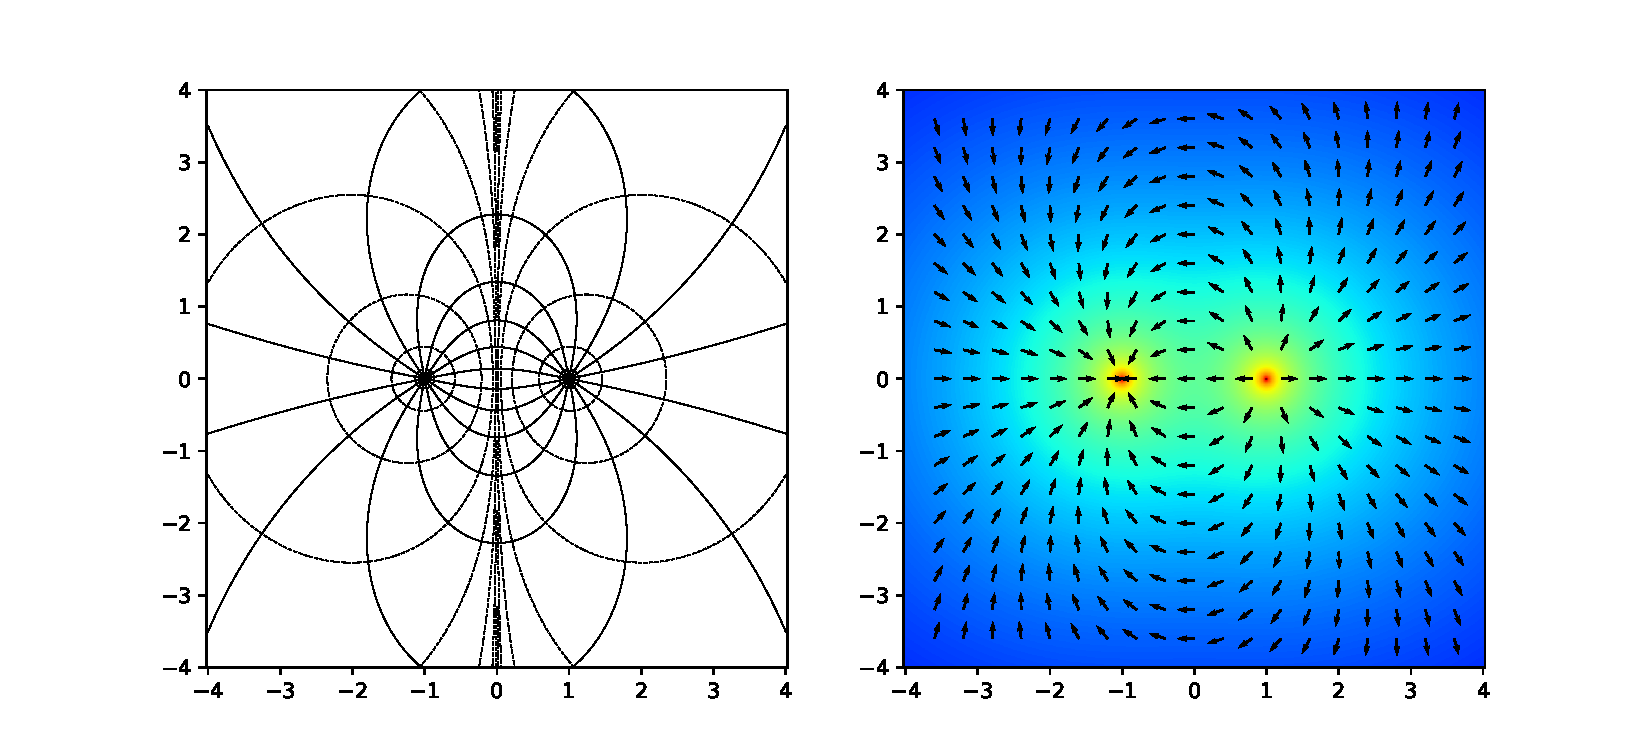
\includegraphics[width=8.2cm]{1.png}}
        \subfigure[电偶极子]{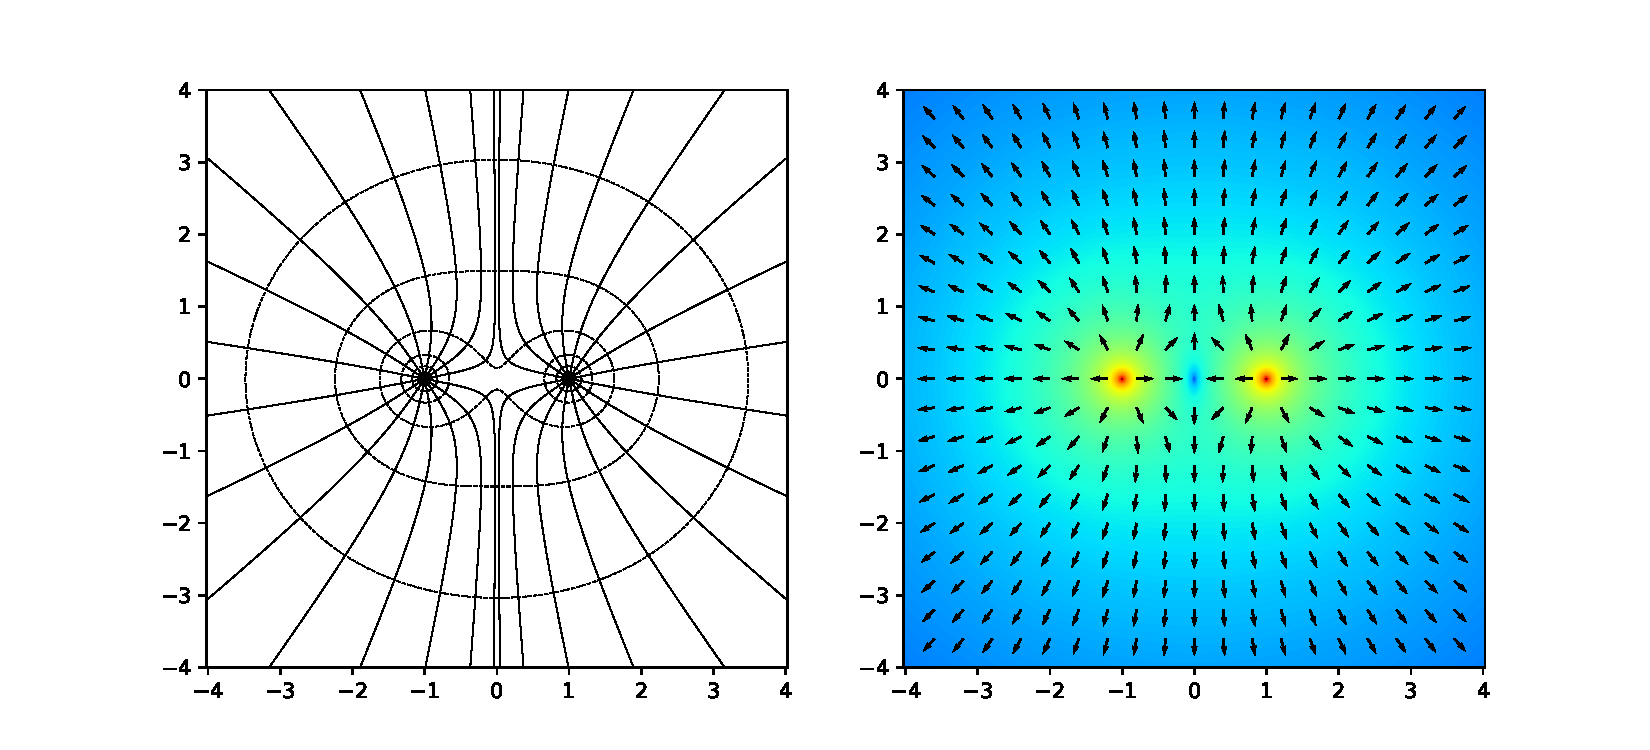
\includegraphics[width=8.2cm]{2.png}}
        \\
        \subfigure[细长带电棒]{\includegraphics[width=8.2cm]{3.png}}
        \subfigure[多个带电棒]{\includegraphics[width=8.2cm]{4.png}}
    \end{center}
    \caption{二维点电荷分布及连续体电荷分布的数值计算电场可视化}
    \label{F2}
\end{figure}

\subsection{连续体电荷分布}
求解区域以及迭代参数与点电荷分布的数值实验设置相同,放置一根长0.8,中心位于原点的沿$x$方向的带电细棒,电荷密度为$\rho/(\varepsilon h_x h_y)=1$,边界条件设置为电势为零,即(\ref{2.1a})(\ref{2.1b})式,电场的计算结果如图\ref{F2}(3)所示。在相同的求解参数下,求解三根带电细棒在有限空间中的电场分布,计算结果如图\ref{F2}(4)所示,第一、二根细棒长0.6,沿$y$轴方向,电荷密度为$\rho/(\varepsilon h_x h_y)=1$,中心分别位于$(-0.4,0.3),(0.4,0.3)$处,第三根细棒长0.8,沿$x$轴方向,电荷密度为$\rho/(\varepsilon h_x h_y)=-2$,中心位于$(0,-0.6)$。数值实验的结果符合静静电场规律,在边界处电场方向垂直与边界,在带电帮附近,电场方向几乎垂直与细棒。

\section{讨论}
本文报告了一种数值求解泊松方程的方法,并举例与单网格算法相比,说明了其高效性与实用性,可视化图像也清晰的展现出了求解结果。目前对于该方法的讨论还不够全面,对于其在一些复杂的电荷分布的可用性还待进一步论证。目前所运用的多重网格方法循环模式是最基础的V循环,还有F循环和W循环在特定条件下会展现出更快的收敛速度。对于插值算法,报告的方法中采用的是最简单的双性插值,从图\ref{F1}(b)可以看出插值的误差还处于一个较低的水准,每次提升网格精度都会导致误差大幅度的提高,可以看到在蓝色折线的第二个点与第八个点都有急剧的误差升高现象,这是由于插值不够平滑所带来的,可以考虑运用双三次插值的方法进行插值,可以在细化网格时获得更低的误差值。

多重网格方法作为预调节器,除了可以用来提高偏微分方程的求解速度以外,对于其他的线性系统,乃至非线性系统的迭代提速,降低误差都有很大的实用价值。对于一般的非稀疏线性方程组,可以配合连续过松弛迭代方法进行求解,同样可以获得十分可观的结果。

\section{附录}
本文二维正弦电荷分布的数值求解的完整Python代码如下,其余的代码可以通过公开的GitHub数据库查看\url{https://github.com/812610357/Electrodynamics},欢迎标星收藏跟随关注。

\begin{lstlisting}
    import time
    import matplotlib.pyplot as plt
    import numpy as np
    import pandas as pd
    from scipy import sparse
    
    ######## 设置求解参数 ########
    postIterError = 1e-10  # 后平滑共轭梯度迭代误差
    mainIterTimes = 3    # 多重网格迭代次数,即网格粗化等级
    preIterTimes = 3   # 预平滑共轭梯度迭代次数
    error = np.array([])
    
    ######## 定义求解区域 ########
    xMin = -1
    xMax = 1
    yMin = -1
    yMax = 1
    d = np.array([1e-3, 1e-3])  # [y,x]
    x = np.arange(xMin, xMax+d[1], d[1])
    y = np.arange(yMin, yMax+d[0], d[0])
    xx, yy = np.meshgrid(x, y)
    
    ######## 定义电荷分布 ########
    epsilon0 = 1
    rho = 2*np.pi**2*np.sin(np.pi*xx)*np.sin(np.pi*yy)
    
    ######## 多重网格-五点差分-共轭梯度-求解泊松方程 ########
    t = time.time()
    
    
    def smoothing(phi, f, d, pre=False):
        '''
        平滑算子,共轭梯度迭代,返回迭代结果和剩余误差
        '''
        size = np.array(f.shape, dtype='int')
    
        def coefficientMatrix():
            '''
            展平到一维空间,根据五点差分法,使用稀疏矩阵,初始化系数矩阵
            '''
            #### 主对角线 ####
            C = np.ones(sizeA)*-2*(1/d[1]**2+1/d[0]**2)
            #### x方向差分 ####
            Dx = np.ones(sizeA-1)/d[1]**2
            Dx[np.arange(1, size[0], 1, dtype='int')*size[1]-1] = 0
            #### y方向差分 ####
            Dy = np.ones(sizeA-size[1])/d[0]**2
            A = sparse.diags([C, Dx, Dx, Dy, Dy], [0, 1, -1, size[1], -size[1]])
            return A
    
        def leftBoundary(phi):
            '''
            x=xMin,左侧一类边值条件
            '''
            b[:size[1]] = phi
            A.data[0, :size[1]] = 1
            A.data[[1, 2], :size[1]] = 0
            A.data[3, :size[1]*2] = 0
            pass
    
        def rightBoundary(phi):
            '''
            x=xMax,右侧一类边值条件
            '''
            b[-size[1]:] = phi
            A.data[0, -size[1]:] = 1
            A.data[[1, 2], -size[1]:] = 0
            A.data[4, -size[1]*2:] = 0
            pass
    
        def bottomBoundary(phi):
            '''
            y=yMin,下侧一类边值条件
            '''
            b[np.arange(size[0])*size[1]] = phi
            A.data[0, np.arange(size[0])*size[1]] = 1
            A.data[1, np.arange(size[0])*size[1]+1] = 0
            A.data[3, np.arange(size[0])*size[1]] = 0
            A.data[4, np.arange(size[0])*size[1]] = 0
            pass
    
        def topBoundary(phi):
            '''
            y=yMax,上侧一类边值条件
            '''
            b[np.arange(size[0])*size[1]-1] = phi
            A.data[0, np.arange(size[0])*size[1]-1] = 1
            A.data[2, np.arange(size[0])*size[1]-2] = 0
            A.data[3, np.arange(size[0])*size[1]-1] = 0
            A.data[4, np.arange(size[0])*size[1]-1] = 0
            pass
    
        def conjGradMethod(A, b, x):
            '''
            共轭梯度迭代求解
            '''
            global error
            r = b - sparse.dia_matrix.dot(A, x)
            d = r
            CGMstep = 0
            while CGMstep < size[0]*size[1]:
                Ad = sparse.dia_matrix.dot(A, d)
                alpha = np.dot(r.T, r) / np.dot(d.T, Ad)
                x = x + alpha*d
                beta = np.dot((r - alpha*Ad).T, r - alpha*Ad) / np.dot(r.T, r)
                r = r - alpha*Ad
                d = r + beta*d
                CGMstep += 1
                Error = np.linalg.norm(r, ord=np.inf)  # 后向误差
                print('VMGstep=%d,CGMstep=%d,log(r)=%6f' %
                      (VMGstep, CGMstep, np.log10(Error)))
                error = np.append(error, Error)  # 存储余项误差数据
                if pre and CGMstep >= preIterTimes:  # 预迭代次数上限
                    break
                if Error < postIterError:  # 误差上限
                    break
            return x
    
        ######## 组装求解矩阵 ########
        sizeA = size[0]*size[1]
        A = coefficientMatrix()
        b = np.reshape(f, (sizeA, 1))
    
        ######## 定义边界条件 ########
        leftBoundary(0)
        rightBoundary(0)
        bottomBoundary(0)
        topBoundary(0)
    
        ######## 解线性方程组 ########
        phi = np.reshape(phi, (sizeA, 1))  # 展平到一维空间
        phi = conjGradMethod(A, b, phi)
    
        ######## 计算剩余误差 ########
        res = b-sparse.dia_matrix.dot(A, phi)
        phi = np.reshape(phi, (size[0], size[1]))  # 剩余误差重整回二维空间
        res = np.reshape(res, (size[0], size[1]))  # 求解结果重整回二维空间
    
        return phi, res
    
    
    def restriction(res):
        '''
        限制算子,将网格间距为h的剩余误差投影到间距为2h的网格
        '''
        xi = np.arange(0, res.shape[1]+1, 2, dtype='int')
        yi = np.arange(0, res.shape[0]+1, 2, dtype='int')
        xic = xi[1:-1]
        yic = yi[1:-1]
        xii, yii = np.meshgrid(xi, yi)
        xiic = xii[1:-1, 1:-1]
        yiic = yii[1:-1, 1:-1]
        rhs = np.zeros(((res.shape[0]-1)//2+1, (res.shape[1]-1)//2+1))
        rhs[1:-1, 1:-1] = (4*res[xiic, yiic]+2*(res[xiic-1, yiic]+res[xiic+1, yiic]+res[xiic, yiic-1]+res[xiic, yiic+1]) +
                           res[xiic-1, yiic-1]+res[xiic-1, yiic+1] + res[xiic+1, yiic+1]+res[xiic+1, yiic-1])/16  # 非边界
        rhs[1:-1, 0] = (2*res[yic, 0]+res[yic-1, 0]+res[yic+1, 0])/4  # 左边界
        rhs[1:-1, -1] = (2*res[yic, -1]+res[yic-1, -1]+res[yic+1, -1])/4  # 右边界
        rhs[0, 1:-1] = (2*res[0, xic]+res[0, xic-1]+res[0, xic+1])/4  # 下边界
        rhs[-1, 1:-1] = (2*res[-1, xic]+res[-1, xic-1]+res[-1, xic+1])/4  # 上边界
        rhs[[0, 0, -1, -1], [0, -1, 0, -1]] = res[[0, 0, -1, -1], [0, -1, 0, -1]]  # 四个角
        return rhs
    
    
    def prolongation(eps):
        '''
        延拓算子,将网格间距为2h的低精度解插值到间距为h的网格
        '''
        xi = np.arange(0, eps.shape[1], 1, dtype='int')
        yi = np.arange(0, eps.shape[0], 1, dtype='int')
        xic = xi[:-1]
        yic = yi[:-1]
        xii, yii = np.meshgrid(xi, yi)
        xiic = xii[:-1, :-1]
        yiic = yii[:-1, :-1]
        phi = np.zeros(((eps.shape[0]-1)*2+1, (eps.shape[1]-1)*2+1))
        phi[xii*2, yii*2] = eps[xii, yii]  # 非插值点
        phi[xiic*2+1, yiic*2+1] = (eps[xiic, yiic]+eps[xiic+1, yiic] +
                                   eps[xiic+1, yiic+1]+eps[xiic+1, yiic+1])/4  # 中心点
        phi[xiic*2+1, yiic*2] = (eps[xiic, yiic]+eps[xiic+1, yiic])/2  # 左右点
        phi[yic*2+1, -1] = (eps[yic, -1]+eps[yic+1, -1])/2
        phi[xiic*2, yiic*2+1] = (eps[xiic, yiic]+eps[xiic, yiic+1])/2  # 上下点
        phi[-1, xic*2+1] = (eps[-1, xic]+eps[-1, xic+1])/2
        return phi
    
    
    def VCycleMultiGrid(phi, f, d):
        '''
        V循环多重网格法主程序
        '''
        global VMGstep
        phi, res = smoothing(phi, f, d, pre=True)  # 预平滑
        rhs = restriction(res)
        eps = np.zeros_like(rhs)
        VMGstep += 1
        if VMGstep < mainIterTimes:
            VCycleMultiGrid(eps, rhs, 2*d)
        else:
            eps = smoothing(eps, rhs, 2*d, pre=True)[0]  # 到达最大主迭代次数
        VMGstep -= 1
        phi += prolongation(eps)
        phi = smoothing(phi, f, d)[0]  # 后平滑
        return phi
    
    
    VMGstep = 1
    phi = np.zeros((len(y), len(x)))  # 等号左侧自变量的预测
    f = -rho/epsilon0                 # 等号右侧的函数表达式
    phi = VCycleMultiGrid(phi, f, d)
    
    ######## 三点差分-计算梯度 ########
    Ex = (phi[1:-1, 2:]-phi[1:-1, :-2])/2/d[1]
    Ey = (phi[2:, 1:-1]-phi[:-2, 1:-1])/2/d[0]
    Exy = -np.stack((Ey, Ex), axis=2)
    print('迭代耗时:%6fs' % (time.time()-t))
    
    ######## 计算误差分析 ########
    phi0 = np.sin(np.pi*xx)*np.sin(np.pi*yy)/epsilon0  # 该系统的解析解
    rms = np.linalg.norm(np.reshape(
        phi-phi0, (phi.size, 1)), ord=2)/np.sqrt(phi.size)  # 均方根误差
    print('均方误差:%e' % rms)
    dataframe = pd.DataFrame(data={'error': error})  # 导出迭代余项误差
    dataframe.to_csv("error.csv", index=False, mode='w', sep=',')
    
    ######## 电势电场求解误差的可视化 ########
    
    
    def plotElectricPotential():
        '''
        绘制电势大小
        '''
        plt.pcolor(x, y, phi, cmap='jet')
        plt.colorbar()
        plt.xlabel('X')
        plt.ylabel('Y')
        plt.title('Potential distribution')
        pass
    
    
    def plotEquipotentialSurface():
        '''
        绘制等势线
        '''
        plt.contour(x, y, phi, 10, colors='k',
                    linestyles='dashed', linewidths=0.5)
        pass
    
    
    def plotElectricFieldIntensity():
        '''
        绘制电场强度大小
        '''
        E = np.linalg.norm(Exy, ord=2, axis=2)
        E[200-1, 300-1:701-1] = np.NaN
        E[500-1:801-1, 300-1] = np.NaN
        E[500-1:801-1, 700-1] = np.NaN
        plt.pcolor(x[1:-1], y[1:-1], E, cmap='jet')
        plt.colorbar()
        plt.xlabel('X')
        plt.ylabel('Y')
        plt.title('Field distribution')
        pass
    
    
    def plotElectricFieldDirection():
        '''
        绘制电场强度方向
        '''
        xi = np.arange(0, 20, 1, dtype='int') * (len(x)-1)//20+(len(x)-1)//40
        yi = np.arange(0, 20, 1, dtype='int') * (len(y)-1)//20+(len(y)-1)//40
        xii, yii = np.meshgrid(xi, yi)
        xa = x[xi]
        ya = y[yi]
        E = np.linalg.norm(Exy[yii-1, xii-1, :], ord=2, axis=2)
        dx = Exy[yii-1, xii-1, 1]/E
        dy = Exy[yii-1, xii-1, 0]/E
        plt.quiver(xa, ya, dx, dy)
        pass
    
    
    plt.figure(figsize=(10, 8))
    plt.subplot(2, 2, 1)
    plt.axis('equal')
    plt.axis([-1, 1, -1, 1])
    plotElectricPotential()
    plotEquipotentialSurface()
    plt.subplot(2, 2, 2)
    plt.axis('equal')
    plt.axis([-1, 1, -1, 1])
    plotElectricFieldIntensity()
    plotElectricFieldDirection()
    plt.subplot(2, 1, 2)  # 绘制误差下降曲线
    plt.yscale('log')
    plt.plot(error)
    plt.xlabel('Iterating times')
    plt.ylabel('Residual errors')
    plt.title('Residual errors')
    plt.show()
    
\end{lstlisting}

\end{document}